\documentclass{standalone}

\usepackage{circuitikz}

\begin{document}

% INT_AY21_L20_Fig03_Ang_mom_variations.png

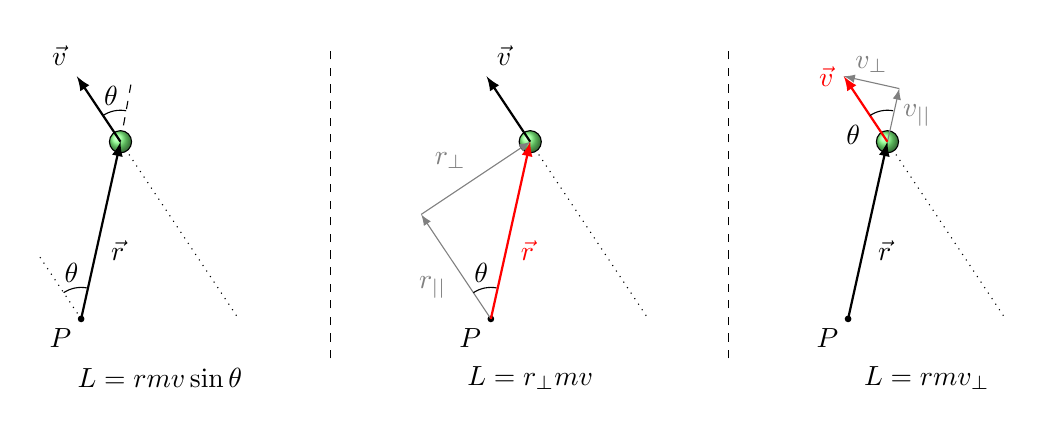
\begin{tikzpicture}[> = latex]
\matrix[column sep = 1 cm]{

	% Marked point
	
	\draw [fill = black] (0, 0) circle (1 pt) node [below left] {$P$};
	
	% Line of motion
	
	\draw [dotted] (0, 3) -- (2, 0);
	
	% Angle indicators
	
	\draw [dotted] (0, 0) -- ++ ({180 - atan(1.5)} : 1);
	\draw ({180 - atan(1.5)} : 0.4) arc ({180 - atan(1.5)} : {atan(5.5)} : 0.4);
	\node at ({90 + 0.5 * (atan(5.5) - atan(1.5))} : 0.6) {$\theta$};
	
	\draw [dashed] (0.5, 2.25) -- ++ ({atan(5.5)} : 0.75);
	\draw (0.5, 2.25) ++ ({atan(5.5)} : 0.4) arc ({atan(5.5} : {180 - atan(1.5)} : 0.4);
	\node at (0.3783, 2.838) {$\theta$};
	
	% Object
	
	\draw [ball color = green!50] (0.5, 2.25) circle (4 pt);
	
	% Position, velocity vectors
	
	\draw [->, thick] (0.5, 2.25) -- ++ ({180 - atan(1.5)} : 1) node [above left] {${\vec v}$};
	\draw [->, thick] (0, 0) -- node [below right] {${\vec r}$} (0.5, 2.25);
	
	% Label
	
	\node at (1, -0.75) {$L = rmv \sin \theta$};
	
&

	\draw [dashed] (0, -0.5) -- (0, 3.5);
	
&

	% Marked point
	
	\draw [fill = black] (0, 0) circle (1 pt) node [below left] {$P$};
	
	% Line of motion
	
	\draw [dotted] (0, 3) -- (2, 0);
	
	% Object + velocity vector
	
	\draw [ball color = green!50] (0.5, 2.25) circle (4 pt);
	\draw [->, thick] (0.5, 2.25) -- ++ ({180 - atan(1.5)} : 1) node [above right] {${\vec v}$};
	
	% Position vector components

	\draw [->, gray] (0, 0) -- node [below left] {$r_{||}$} (-0.8850, 1.327);
	\draw [->, gray] (-0.8850, 1.327) -- node [above left] {$r_\perp$} (0.5, 2.25);
	\draw [->, red, thick] (0, 0) -- node [below right] {${\vec r}$} (0.5, 2.25);
	
	% Angle indicator
	
	\draw ({180 - atan(1.5)} : 0.4) arc ({180 - atan(1.5)} : {atan(5.5)} : 0.4);
	\node at ({90 + 0.5 * (atan(5.5) - atan(1.5))} : 0.6) {$\theta$};
	
	% Label
	
	\node at (0.5, -0.75) {$L = r_\perp mv$};
	
&

	\draw [dashed] (0, -0.5) -- (0, 3.5);
	
&

	% Marked point
	
	\draw [fill = black] (0, 0) circle (1 pt) node [below left] {$P$};
	
	% Line of motion
	
	\draw [dotted] (0, 3) -- (2, 0);
	
	% Object + position vector
	
	\draw [ball color = green!50] (0.5, 2.25) circle (4 pt);
	\draw [->, thick] (0, 0) -- node [below right] {${\vec r}$} (0.5, 2.25);
	
	% Velocity vector components
	
	\draw [->, gray] (0.5, 2.25) -- node [right] {$v_{||}$} (0.6498, 2.925);
	\draw [->, gray] (0.6498, 2.925) -- node [above] {$v_\perp$} (-0.05480, 3.082);
	\draw [->, thick, red] (0.5, 2.25) -- ++ ({180 - atan(1.5)} : 1) node [left] {${\vec v}$};
	
	% Angle indicator
	
	\draw (0.5, 2.25) ++ ({atan(5.5)} : 0.4) arc ({atan(5.5} : {180 - atan(1.5)} : 0.4) node [below left] {$\theta$};
	
	% Label
	
	\node at (1, -0.75) {$L = rmv_\perp$};

\\	
};

\end{tikzpicture}

\end{document}